\subsection{Trådløs kommunikation}\label{sec:traadloes_komm_design}
For at kommunikere trådløst benyttes Cypress BLE modul. Kommunikationstypen BLE \citep{cypressguide2014} er en energi-effektiv variation af Bluetooth-teknologi. Bluetooth er en standard for kortdistance trådløs teknologi, som muliggør kommunikation mellem flere enheder via radiobølger. Dette betyder, at systemet anvender mindre batteri på Bluetooth-kommunikationen, end på almindelig Bluetooth. Af denne grund kan der benyttes små batterier, uden det bliver nødvendigt at skifte dem ofte \citep{gupta2013}. 


\begin{figure}[H]
	\centering
	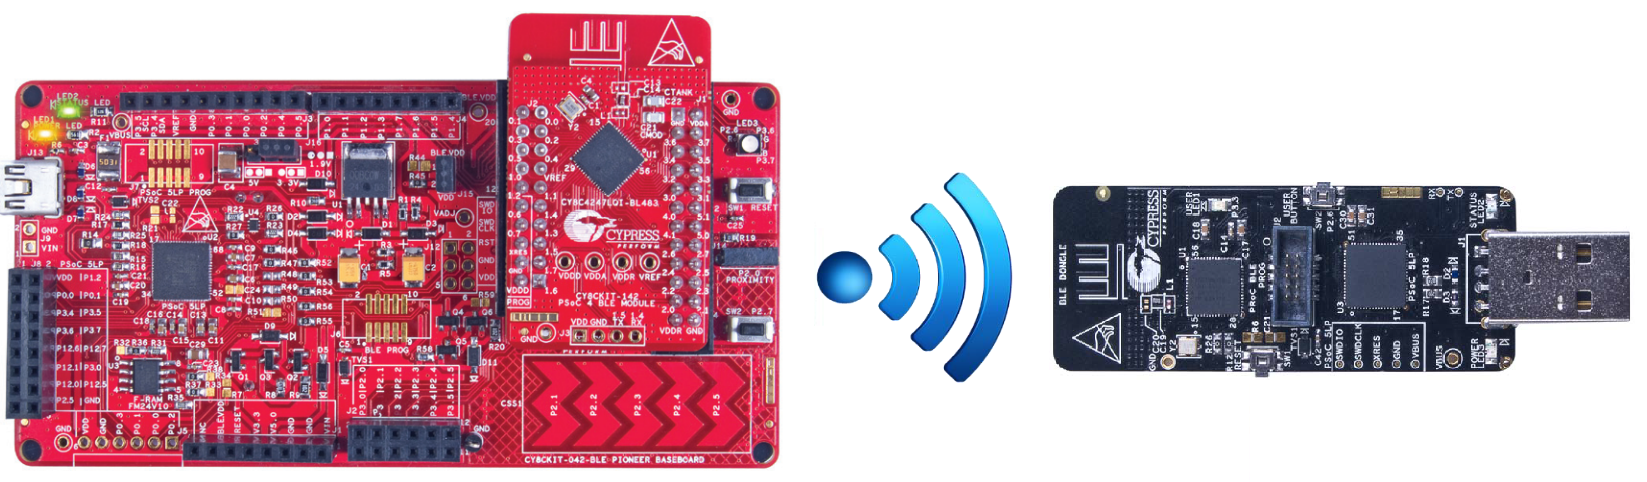
\includegraphics[width=1\textwidth]{figures/BLEToBLEdongle}
	\caption{Illustration af kommunikation mellem mikrokontroller og BLE dongle \citep{cypresspsoc2015, cypressguide2014}.}
	\label{fig:BLE_to_BLE_Dongle}
\end{figure}

\noindent
Til det endelige system benyttes der udover mikrokontrolleren også en BLE-dongle. Dette er etableret for at tillade trådløst kommunikation mellem en computer og mikrokontrolleren, hvortil en illustration kan ses af \autoref{fig:BLE_to_BLE_Dongle}. Dette tillader således trådløs test, visualisering, og debugging af mikrokontrolleren. BLE-donglen forsynes via USB-porten på den givne computer med $5~V$ \citep{cypressguide2014}. Denne form for BLE-kommunikation anvendes for at kommuinkere trådløst med en computer, således en visualisering er mulig. For at systemet senere skal kunne anvendes til ALS-patienter med gang, skal der tages højde for en maksimal forsinkelse, for at systemet kan følge almindelig gang. Gangfunktionen for ALS-patienter varierer alt efter, hvor mange funktioner der er nedsat, eksempelvis vil patienter med luftvejsproblemer gå langsommere. ALS-patienter har en gennemsnitlig gangfunktion på $1,02~m/s$ \citep{hausdorff2000}, hvorfor en forsinkelse på 100 ms vurderes at være acceptabel. Da systemet skal placeres på benet, vurderes det at en kommunikationsrækkevidde på $2~m$ er tilstrækkeligt.
\\

\textbf{Krav:}
\begin{itemize}
\item Mikrokontrolleren skal kommunikere trådløst med en computer
\item BLE-dongle skal forsynes via USB
\item Skal have en maksimal forsinkelse på 100 ms \fxnote{skal denne forsinkelse være større eller mindre?? - HUSK at ændre i brødteksten også!}
\item Skal have en kommunikationsrækkevidde på $2~m$
\end{itemize}